\chapter{Predict Water Body from Low-Resolution Satellite Images}
\label{chap-4-predict-water-body}
\begin{ChapAbstract}
In this chapter, we present our research on predicting the next MODIS images on Tonlesap lake, especially concerning on water body and shoreline of the lake, and then use this prediction to estimate the futur water area of this lake.
\end{ChapAbstract}

\section{Introduction}
Deep learning methods exhibit promising performance for the very close problem of ours: video frame prediction. However, directly adoption of these methods maynot result in a sufficient result in satellite image band prediction, due to  limitations below:
\begin{enumerate} 
    \item Hydrological status is commonly a annually periodical phenomenon. On the other hand, video frame prediction is more focused on objects' movement. Therefore, we need a paradigm which makes used of more efficiently the periodical characteristic.
    \item These methods don't focus on lake's water body which is the main element in this work. A good forecasting in the land region around the lake incorporated with a bad prediction in lake' s water body may cheat us by the metric evaluated on the whole image, such as MSE, MAE, SSIM, PSNR, \dots 
\end{enumerate}
In this chapter, we develop a model that uses the MODIS NDVI-band data until timesteps $t$ to predict the MODIS NDVI-band at timesteps $t+1$ with a greater concern in boundary of the lake. Traditional recurrent neural networks only use a fixed-length sequence of $(x_{t - l + 1}, x_{t - l + 2},\dots,x_{t})$, where $l$ is the sequence length to predict $x_{t + 1}$. It eases to suffer vanishing gradient problem. Although some advanced recurrent neural networks, such as GRU, LSTM, \dots, are proved to help to reduce this issue, the computational cost is still unecessarily large. Indeed, the annual periodity of hydrological status lead to the length of input sequence should be at least 46 (46 is the number of MODIS Terra and Aqua in one year). Loading all of these sequences to GPU wastes a large amount of resource, because each data in the input sequence is used only one time in the forward pass. 
We have addressed these limitations using a neural network model which is the fusion of ConvLSTM and Attention mechanism. Instead of directly using a unique long sequence as input, our model divides data into multiple small/medium length sequences in both long-term and short-term time dependency. The ConvLSTM-based neural networks have the goal of extracting the latent representations of both long and short-term time dependency. Then the attention mechanism is adpoted to summary these two time latent information. Finally, a ConvLSTM network part is used to produce the final prediction.

\section{Data}
\subsection{Study Domain}
This study focuses on the Tonlesap lake, which is a seasonally inundated freshwater lake in in the central lowlying territory of the Cambodia. Our study site was defined by a rectangular boundary of (13.53°N, 103.12°E), (12.42°N, 104.61°E). The Tonlé Sap watershed usually experiences two
monsoon periods, dry season from December to April and rainy from
May to October. %cite (MRC/WUP, 2006)%
The total open water area, including seasonal inundated wetland, varies from 2500 $km^2$ in the driest month (April) to a maximum of 14,500 $km^2$ during flood season (September and October). Fig %Fig label%
depicts the study area in January 2017.

This great lake functions as a natural reservoir for the Mekong River
system during dry season, and regulates flood discharge during wet
season. Flood pulse, as a succession of periodic flooding, is the most
notable feature of the Tonlé Sap Lake. During the dry season, a slow
release of the lake water flows into the Mekong through the Tonlé Sap
River; then the lake is refilled by a reverse water flow from the Mekong
during monsoon season, hence forming a globally unique hydrodynamic pattern in the Mekong watershed. %cite (Sarkkula et al., 2008)%

\subsection{Satellite Observations}
\label{subsection-used-data}
% 

%
%\section{Related Work}
%\textbf{Satellite Image Prediction} Several pioneering approaches have explored the task of predicting the next satetllite image(s) by neural networks %cite%. 
%Most of these approaches based on Convolutional Long-Short Term Memory (ConvLSTM) as the core architectural element for generating next satellite images. 

\section{Methodology}
\subsection{Data preparation}
As aforementioned, deep-learning based models for prediction require a huge amount of data. In order to meet that demand, we propose a data augmentation procedure in the data pipeline before training and validation phase. The procedure is briefly described as: First MODIS Terra/Aqua images of band NDVI are selected and scaled to $(0,1)$ by max-min normalization. Each sequence of images has the length of 29, where the length for input data is 24 and 5 is the length of prediction output. The number of sequence for training, validation and testing is 528, 46, 83 respectively. Terra and Aqua images are used separately. For each sequence of training and validation set, the last image of input part is chosen for extracting lake boundary. In the set of points of the extracted lake boundary, 32 points are selected, in the manner of nearly equidistance, to be the center of each image patches. Each patch has the size of $32 { x } 32$. Then 30-32 sequence patches of length 53, whose centers are these points, are extracted from the original sequence (the number of patches depends whether the center point can generate a $32 { x } 32$ patch totally inside the image). Finally, each sequence is augmented by four rotation of 90 degree with 2 noise additions (each noise is a tensor of random numbers drawn from a normal distribution with zero mean and 0.1 standard deviation) to generate 11 new sequences (so the number of sequence increases 12 times). In brief, there are 193512, 16920 sequences for training and validation. For testing phase, we inference on whole $513 { x } 513$ image sequences. The procedure is described in detail by the algorithms below:

\begin{algorithm}
    \caption{gen\_data}
    \begin{algorithmic}[1]
        \Inputs{\begin{itemize}
            \item{$(\tX, \tY)$: Tuple of two tensors (input and label) with shape ($IN\_LENGTH, H, W$), and ($OUT\_LENGTH, H, W$)} 
            \item{$water\_threshold$: Double scalar which is threshold of pixel value to be considered as water}
            \item{$patch\_size$: Integer scalar which is size of each patch}
        \end{itemize}}
        \Outputs{$\tX_1, \tY_1$: Tuple of output tensors (input and label) with shape ($NUM\_PATCHES, IN\_LENGTH, patch\_size, patch\_size)$, ($NUM\_PATCHES, OUT\_LENGTH, patch\_size, patch\_size$)}
        
        \State $last\_inputs \gets \tX[-1]$
        \State{$boundary\_mask\_lake \gets$ find\_boundary\_mask\_lake(
            \Statex \hspace{10mm}$last\_inputs, water\_threshold$)}
        \State $list\_center\_pos \gets$ get\_center\_pos($boundary\_mask\_lake$)
        \Returns{get\_patches($\tX, list\_center\_pos$), get\_patches($\tY, list\_center\_pos$)}
    \end{algorithmic}
\end{algorithm}

\begin{algorithm}
    \caption{find\_boundary\_mask\_lake}
    \begin{algorithmic}[1]
        \Inputs{\begin{itemize}
            \item{$(\tX)$: Tensor with shape ($H,W$)}
            \item{$water\_threshold$: Double scalar which is threshold of pixel value to be considered as water}
        \end{itemize}}
        \Outputs{$\tM$: 0-1 Tensor, with shape ($H,W$): Mask tensor, 1 if pixel is on lake boundary and 0 otherwise}
        
        \State $\tX_1 \gets$ mask\_lake\_img($\tX, water\_threshold$)
        \Returns{find\_boundaries($\tX_1$)}
    \end{algorithmic}
\end{algorithm}

%
%\begin{algorithm}
%    \caption{mask\_lake\_img}
%    \begin{algorithmic}[1]
%    \end{algorithmic}
%\end{algorithm}


\subsection{Prreliminaries on Neural Attention Models}

\subsection{Model}
Our model mainly consists of 3 parts: Short-term temporal dependency, Periodically Shifted Attention Mechanism and the Jointly Training.  

We define some parameters for the model:
\begin{itemize}
    \item $S$: The number of data in a period,
    \item $SL$: Sequence input length of short-term part,
    \item $P$: The number of years for attention mechanism,
    \item $Q$: The number of relevant timesteps in a year for attention. Q is prefered to be odd,
    \item $FL$: The number of last images of timesteps $t$ used as short term-length features for data of timesteps $t$,
    \item $FH$: The number of previous years images of timesteps $t$ used as historical features for data of timesteps $t$. These images have the same indices in their periods as that of image at timesteps $t$ ($t-S, t-2S,\dots$).
\end{itemize}
Let $W, H$ is the shape of an image, $\tX$ is the set of image at each timesteps from past to present. 

\subsubsection{Model input preparation}
The model has four inputs, each input is a tensor. Two of them are used for short-term part and the remains are used for long-term part. These inputs can be described in detail as: At timesteps $t$, the label is the image at timesteps $t + 1$, the inputs consist of (for simplicity, batch size is set to 1):
\begin{itemize}
    \item short-term CNN feature $\tX1$: a tensor with shape $(SL, W, H)$. Each $tX1[i,:,:]$ is $\tX[t - SL + 1 + i]$ for $i$ in $[0, SL - 1]$,
    \item short-term LSTM feature $\tX2$: a tensor with shape $(SL, W, H, FH+FL)$. For each $i$ in $[0, SL - 1]$, for each $j$ in $[0, FH - 1]$, $\tX2[i,:,:,j] = \tX[t - SL + 1 + i - (FH - j)*S]$; for each $j$ in $[0, FL - 1]$, $\tX_2[i,:,:,FH + j] = \tX[t - SL + i - FL + j + 2]$,
    \item long-term CNN feature $\tX3$: a tensor with shape $(P, Q, H, W)$. For each $i$ in $[0, P - 1]$, for each $j$ in $[0, Q - 1]$, $\tX3[i,j,:,:] = \tX[t - (P - i)*S + j - Q/2]$, 
    \item long-term LSTM feature $\tX4$: a tensor with shape $P, Q, H, W, FH + FL$. For each $i$ in $[0, P - 1]$, for each $j$ in $[0, Q - 1]$, let $t_{i, j} = t - (P - i)*S + j - Q/2$, $\tX4[i,j, :, :, :]$ is gathered in the same manner as the short-term LSTM feature $\tX2[t_{i,j}]$. 
\end{itemize}
Notice that the smallest image input index is $t - (FH + P)*S - Q/2$, so the smallest timestamp $t$ to be able to create an input is $t_0 = (FH + P)*S + Q/2$.

To clearify the definition of those four inputs, we consider the example bellow. Let $S = 46, SL = 7, P = 3, Q = 3, FL = 4, FH = 3$. $t = t_0 = (FH + P)*S + Q/2 = 277$.
Four inputs of timesteps $t$ are (we only mention the timesteps index):
\begin{itemize}
    \item short-term CNN feature: $\tX1 = [270, 271, 272, 273, 274, 275, 276]$
    \item short-term LSTM feature: $\tX2 = [[132, 178, 224, 266, 267, 268, 269]
        [133, 179, 225, 267, 268, 269, 270]
        [134, 180, 226, 268, 269, 270, 271]
        [135, 181, 227, 269, 270, 271, 272]
        [136, 182, 228, 270, 271, 272, 273]
        [137, 183, 229, 271, 272, 273, 274]
        [138, 184, 230, 272, 273, 274, 275]]$
    \item long-term CNN feature $\tX3 = [[138, 139, 140], [184, 185, 186], [230, 231, 232]]$
    \item long-term LSTM feature $\tX4 = [[0, 46, 92, 134, 135, 136, 137], [1, 47, 93, 135, 136, 137, 138], [2, 48, 94, 136, 137, 138, 139]]
    [[46, 92, 138, 180, 181, 182, 183], [47, 93, 139, 181, 182, 183, 184], [48, 94, 140, 182, 183, 184, 185]]
    [[92, 138, 184, 226, 227, 228, 229], [93, 139, 185, 227, 228, 229, 230], [94, 140, 186, 228, 229, 230, 231]]$ 
\end{itemize}

\subsubsection{Model architecture}
For simplifying symbols, we set batch size $B = 1$ and ignore it in the following description.
\textbf{Short-term Temporal Dependency}
The first input, \textit{short-term CNN feature} $\tX1$ is fed into list of $SL$ 3 $x$ 3 convolution layers with 32 filters. Then each image $\tX1_i$ convolves with convolution layer $i$ to generate a list of tensors with shape $(H, W, 64)$. These tensors are then concatenate to acquire a tensor with shape $(SL, H, W, 64)$, which is called \textit{short\_term\_cnn\_feature}.

The second input, \textit{short-term LSTM feature} $\tX2$, whose shape is $(SL, H, W, FH + FL)$, is concatenate with the output of the previous step, \textit{short\_term\_cnn\_feature}, to output a tensor \textit{short\_term\_concat} with shape $(SL, H, W, FH + FL + 64)$. Then this output tensor is passed to a Convolutional LSTM layer(s) to capture the spatial temporal relationship in the short-term context. Note that the number 64 can be substitute by any integer number, depending on the characteristic of our data. The purpose of these two parts are gather more information from the nearest previous data, because of their close relevance with the target image. Moreover, the additional information from further past isn't used in the manner of extending the input sequence length as usual, but is used to extend the channel dimension. It plays an important role in making used of the periodical characteristic of this data. The latent representation is computed throught:
\[ h_t = RNN(short\_term\_concat_t, h_{t-1}), \] \label{equation-short-term-information}
where $RNN$ is Convolutional LSTM layer(s).

The third input, \textit{long-term CNN feature} $\tX3$ with shape $(P, Q, H, W)$ is handle in the similar way as \textit{short-term CNN feature}, but with the convolutional filter 32, to produce a tensor \textit{long\_term\_cnn\_feature} with shape $(P, Q, H, W, 32)$. 

The fourth input, \textit{long-term LSTM feature} $\tX4$ with shape $(P, Q, H, W, FH + FL)$ is concatenate with \textit{long\_term\_cnn\_feature} and outputs a tensor with shape $(P, Q, H, W, FH + FL + 32)$ which is called \textit{long\_term\_concat}. Similar to \textit{short-term LSTM feature}, the number 32 can be modified as appropriate. Then for each $p$ in $P$, Convolution LSTM layer(s) is used to capture the hidden representation of each the relevant time in each period ${long\_term\_concat}_p$. 

\[ h_t^{p, q} = RNN(long\_term\_concat_t^{p, q}, h_t^{p, q - 1}), \]
where $h_t^{p, q}$ is the representation of time $q$ in previous year $p$ for the predicted time $t$.

By using an attention mechanism, we capture the periodical characteristic and get the weighted representation of each previous year. Formally, the representation of each previous year $h_p^t$ is a average sum of representations in each relevant time $q$, which is computed by:
\[ h_t^p = \sum_{q \in Q}{\alpha_t^{p,q} h_t^{p,q}}, \]
where weight $\alpha_t^{p,q}$ indicates how much the value of $h_t^{p,q}$ contributes to the value of $h_t^p$. A way to compute $\alpha_t^{p,q}$ is computing the softmax of score indicating the similarity between the previous hidden state $h_t^{p,q}$ and the short-term information $h_t$ \eqref{equation-short-term-information}. Let $score(h_t^{p,q}, h_t)$ be the aforementioned similarity, the alignment function \textit{concat} is adopted to compute $score$:
\[ score(h_t^{p,q}, h_t) = v^T\tanh(W_H h_t^{p,q} + W_X h_t + b_X), \]
where $W_H, W_X, b_X and v$ are learnable parameters, $v^T$ denotes the transpose of $v$. Then $\alpha_t^{p,q}$ is formulated as:
\[ \alpha_t^{p,q} = \frac{\exp(score(h_t^{p,q}, h_t))}{\sum_{q \in Q}{\exp(score(h_t^{p,q}, h_t))}} \]
For each previous day $p$, we get the periodic representation $h_t^p$. After that, we adopt another Convolution LSTM layer(s) to summary the long-term periodic information.
\[ \hat{h}_t^p = RNN(h_t^p, \hat{h}_t^{p-1}) \]
The last time $\hat{h}_t^P$ represents the periodic characteristic of temporal data in a shape of $(H, W, F)$, where $F$ is the filter size of the last Convolution LSTM layer to compute $\hat{h}_t^P$.

\textbf{Joint Training}
Long-term periodic information $\hat{h}_t^P$ and short-term information $h_t$ is concatenated to producte $h_t^c$ which consists of both long-term and short-term spatial temporal data. Notice that $h_t^c$ has the shape of $(H, W, F1)$ Finally, a 2D convolution with kernel size 3 and filter 1 is applied to $h_t^c$ to receive the final prediction $\hat{\tX_{t+1}}$.
\[ \hat{\tX_{t+1}} = Conv2D(h_t^c) \]

%\subsection{Loss Function}


%\subsection{Optimization}


\section{Experiments}
We compared performance of our method to Convolution LSTM (ConvLSTM) and a new method in video prediction, PredRNN++ %cite. 

\subsection{Experimental Settings}
\subsubsection{Data Preprocessing and Data Augmentation}

\subsubsection{Implementation Details}
We implement our method with Tensorflow 1.12. %cite
For training the model, we used Adam %cite
with the mini-batch of 8 inputs. The training was done in a machine equipped with Intel Xeon E5-2650, 377GB RAM, one Nvidia Tesla P100 and CUDA 9.0.

\subsubsection{Baselines}
For comparision, we completed the following baseline models:
\begin{itemize}
    \item \textbf{ConvLSTM}: We use four stacked ConvLSTM layers with filter size 128, 64, 64, 1 respectively. 
    \item \textbf{PredRNN++}: We use PredRNN++ with filter size 128, 64, 64, 1 respectively
\end{itemize}

\subsection{Evaluation measures}
\begin{itemize}
    \item \textbf{Mean Squared Error (MSE)} that is the mean squared error of predicted and groundtruth image. It is also the loss function when training our models.
    \item \textbf{Structural Similarity (SSIM)} that is used for measuring the similarity between two images. %cite
    \item \textbf{Root Mean Squared Error of Predicted Water area ($W\_RMSE$)}: because of highly focusing on water body, we use root mean squared error of water area extracted from 2D groundtruth and predict image. Water area is derived by product of the number of the lake and $0.25^2 km^2$, which is pixel size of MODIS Terra/Aqua image data.
    \item \textbf{Normalized Root Mean Squared Error of Predicted Water area ($W\_NRMSE$)} that is simply the normalized version of $W_RMSE$ by dividing $W_RMSE$ by mean of water area array of image test set.
    \item \textbf{True Prediction Ratio} or \textbf{Recall} that is the fraction of the number of pixels that is predicted to be lake's pixel that are successfully retrieved.
    \[ \texttt{recall} = \frac{|\{\texttt{pixels predicted as lake's pixels}\} \cap \{\texttt{lake's pixels}\}|}{|\{\texttt{lake's pixels}\}|} \]
    \item \textbf{False Discovery Rate (FDR)} that is the rate that a pixel predicted as lake's pixel is truly not.
    \[ \texttt{FDR} = \frac{\texttt{number of false predictions}}{]\texttt{total number of predictions}} \]
    \item \textbf{Area under the Precision-Recall Curve (PR\_AUC)} that summarizes a precision-recall curve as the weighted mean of precisions achieved at each threshold, with the increase in recall from the previous threshold used as the weight:
    \[ \texttt{PR\_AUC} = \sum_n{R_n - R_{n-1}}{P_n}, \] %cite average_precision_score sklearn.metrics
    where $P_n$ and $R_n$ are the precision and recall at the nt threshold. PR\_AUC is a better metric for our goal given that the dataset is class-imbalanced. %cite 180 Choi-Dissertation 
\end{itemize}

\subsection{Results}
We evaluate the prediction performance of all models in both term of regression and classification. The regression results are reported in table %cite
and classification results are reported in table. %cite

Table shows that our methods yeild a higher loss and lower structural similarity than the traditional ConvLSTM model. PredRNN++ performs better in short-term prediction, and the results decrease dramatically when the number of prediction steps increases. The under-expected regression scores of our models result from the grid inference method. It divides the image to patches, which makes a huge influence on the overall regression evaluations.

In contrast with the low regression scores, our methods perform better in classification metrics. The different of classification metrics across multiple methods lies principally on the neighbor region of the lake's boundary, rather than the lake's permanent water region and the far outside lake's region. The better performance of our methods demonstrates that they are more suitable for hydrological prediction, which is the primary goal of this work.

The low recall along with the low FDR of PredRNN++ results from the pixel zero prediction in long-term predictions. ACG\_32 archives the second rank in recall, the first rank in FDR and the first rank in PR\_AUC in 1-timestep prediction, showing that ACG\_32 can properly capture the temporal classification of lake's shoreline region. Figure shows mean of metrics of each predicted image at each timesteps (number  in the table is mean across all timesteps in one prediction). ACG\_32 performs better in W\_NRMSE and PR\_AUC almost all timesteps and performs better than ConvLSTM and PredRNN++ in Recall.

\begin{figure}
    \begin{center}
    \begin{tabular}[b]{c}
      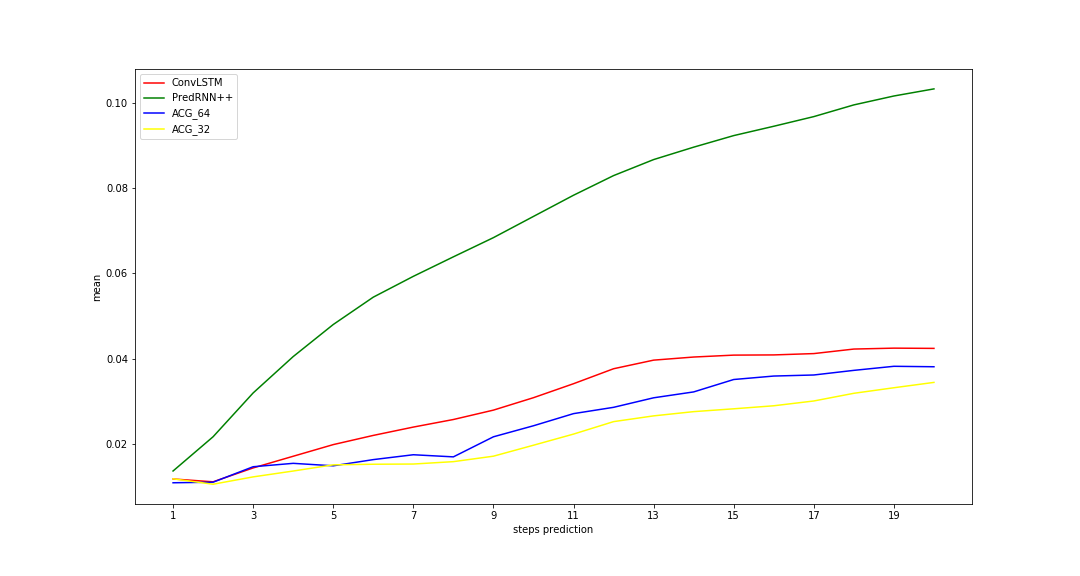
\includegraphics[width=.4\linewidth]{figures/chap4_w_nrmse_timesteps.png} \\
      \small (a) Water NRMSE
    \end{tabular}
    \begin{tabular}[b]{c}
      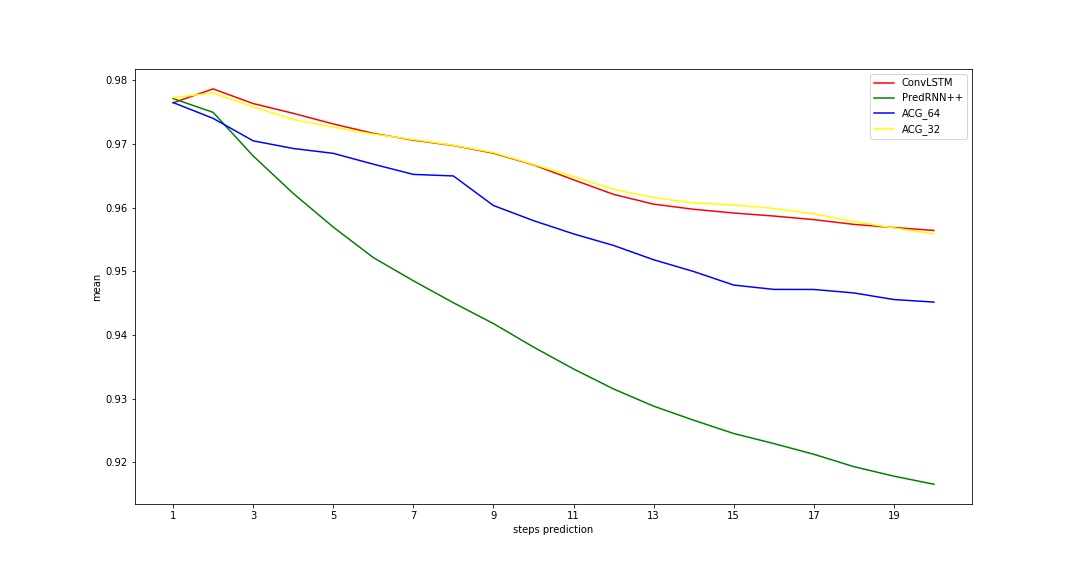
\includegraphics[width=.4\linewidth]{figures/chap4_pr_auc_timesteps.png} \\
      \small (b) PR\_AUC
    \end{tabular}
    \begin{tabular}[b]{c}
        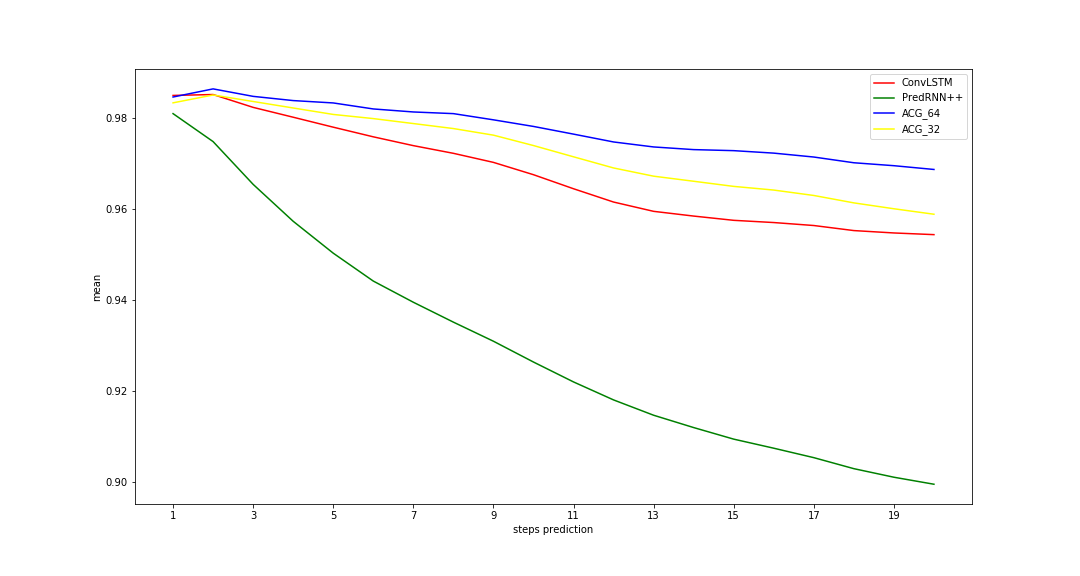
\includegraphics[width=.4\linewidth]{figures/chap4_recall_timesteps.png} \\
        \small (c) Recall
    \end{tabular} 
    \begin{tabular}[b]{c}
        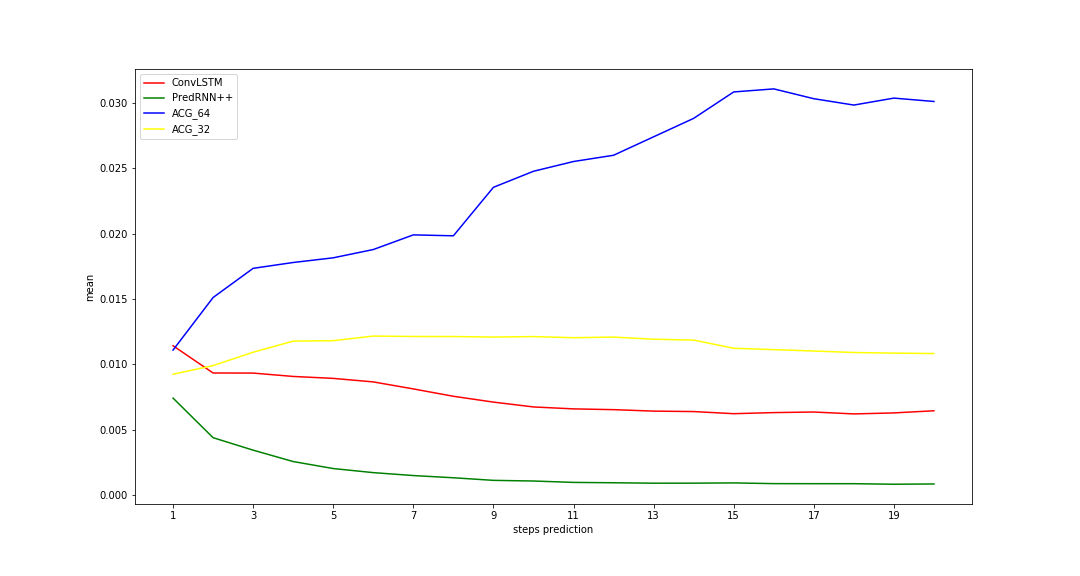
\includegraphics[width=.4\linewidth]{figures/chap4_FDR_timesteps.png} \\
        \small (d) FDR
    \end{tabular}
    \end{center}
    \caption[]{Comparisons of metrics at each timesteps of multiple methods}
    \label{fig:metrics-comparisons-timesteps}
\end{figure}

In Figure \ref{fig:chap4-test-30}, we show an example of the groundtruth and predicted images with metrics plot. Models predict 10 timesteps in the future. This test is at timesteps 241 of year 2016, which is from 21 August to 28 August 2016. As we see in this figure, both attention methods yeild better result in 3 in 4 metrics, except FDR. Especially in long-term prediction, attention-based methods perform better performance. It demonstrates that attention mechanism helps traditional ConvLSTM to remember the periodic characteristic better.  

\begin{figure}
    \begin{center}
        \begin{tabular}[b]{c}
            \small Groundtruth \enspace
            
\includegraphics[width=0.9\textwidth]{figures/chap4/10/30/groundtruth.png} \\
        \end{tabular}
        \begin{tabular}[b]{c}
            \small ConvLSTM \quad
            
\includegraphics[width=0.9\textwidth]{figures/chap4/10/30/convlstm.png} \\
        \end{tabular}
        \begin{tabular}[b]{c}
            \small PredRNN++
            
\includegraphics[width=0.9\textwidth]{figures/chap4/10/30/predrnn_pp.png} \\
        \end{tabular}
        \begin{tabular}[b]{c}
            \small ACG\_64 \qquad
            
\includegraphics[width=0.9\textwidth]{figures/chap4/10/30/attention_clstm_grid.png} \\
        \end{tabular}
        \begin{tabular}[b]{c}
            \small ACG\_32 \qquad
            
\includegraphics[width=0.9\textwidth]{figures/chap4/10/30/attention_clstm_grid_32.png} \\
        \end{tabular}

        \begin{tabular}[b]{c}
            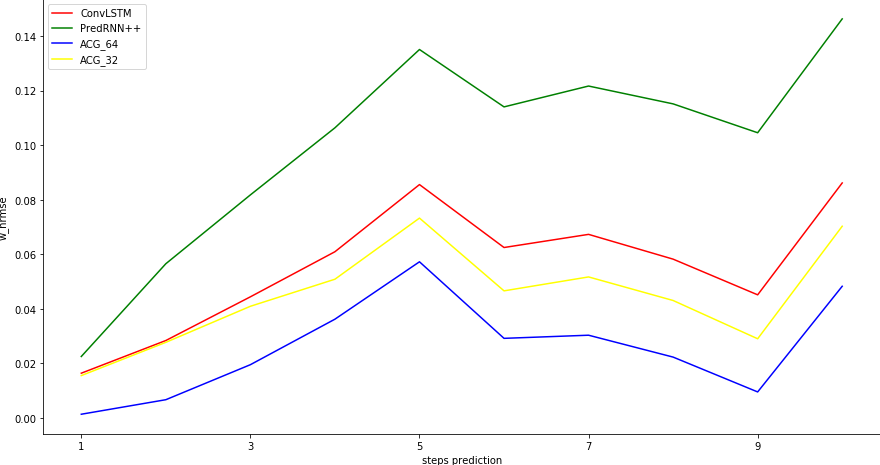
\includegraphics[width=.4\linewidth]{figures/chap4/10/30/w_nrmse.png} \\
            \small Water NRMSE
          \end{tabular}
          \begin{tabular}[b]{c}
            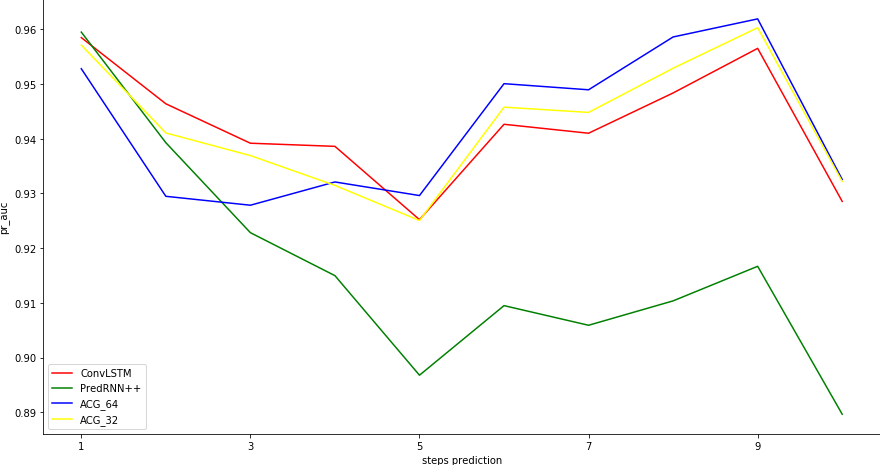
\includegraphics[width=.4\linewidth]{figures/chap4/10/30/pr_auc.png} \\
            \small PR\_AUC
          \end{tabular}
          \begin{tabular}[b]{c}
              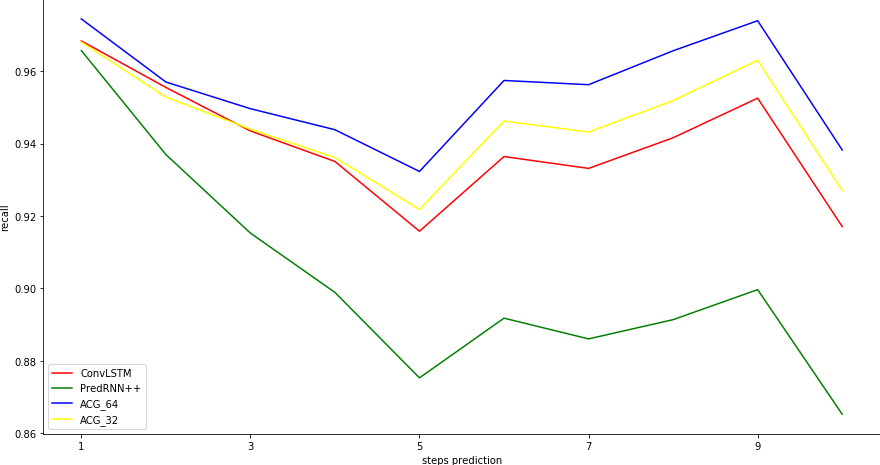
\includegraphics[width=.4\linewidth]{figures/chap4/10/30/recall.png} \\
              \small Recall
          \end{tabular} 
          \begin{tabular}[b]{c}
              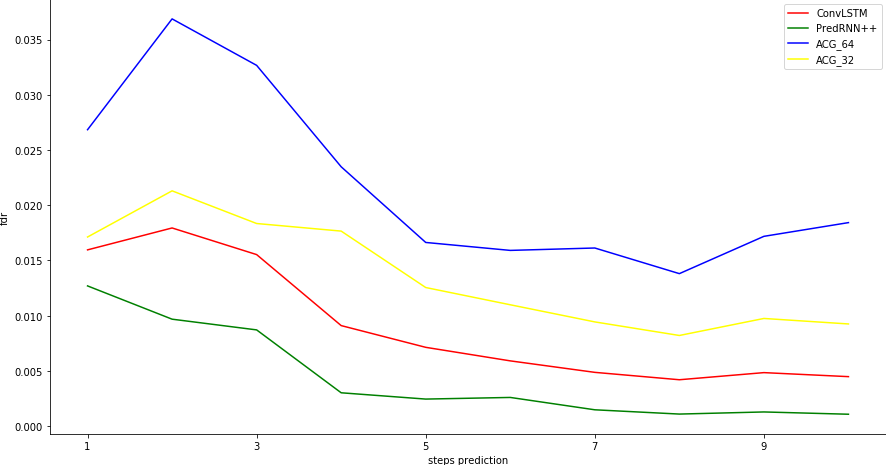
\includegraphics[width=.4\linewidth]{figures/chap4/10/30/fdr.png} \\
              \small FDR
          \end{tabular}
    \end{center}
    \caption[]{Prediction example of multiple methods and groundtruth with metrics}
    \label{fig:chap4-test-30}
\end{figure}


\begin{figure}
    \begin{center}
        \begin{tabular}[b]{c}
            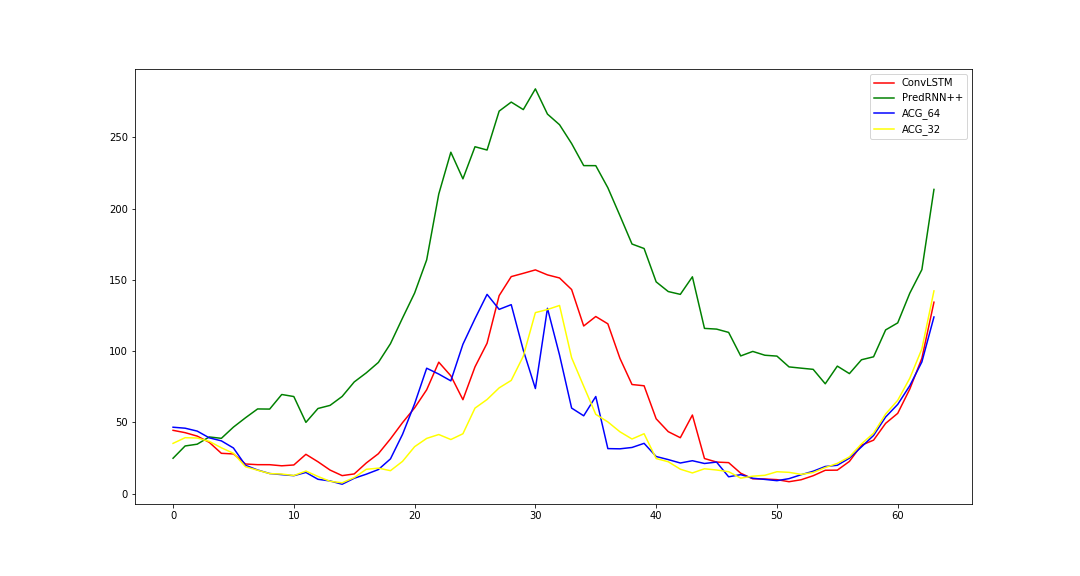
\includegraphics[width=.4\linewidth]{figures/chap4/w_nrmse_all_tests.png} \\
            \small Water NRMSE
          \end{tabular}
          \begin{tabular}[b]{c}
            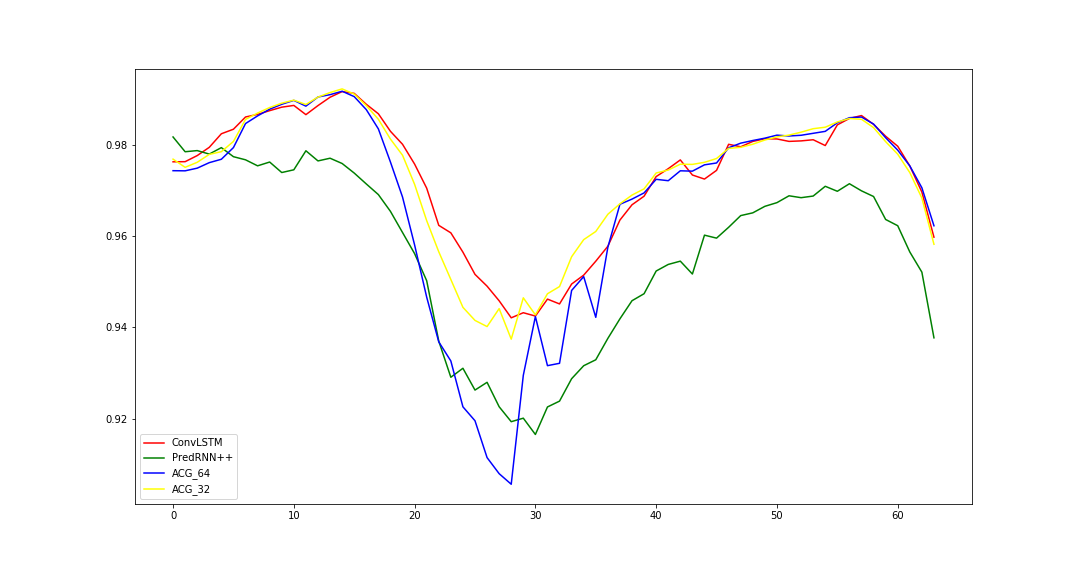
\includegraphics[width=.4\linewidth]{figures/chap4/pr_auc_all_tests.png} \\
            \small PR\_AUC
          \end{tabular}
          \begin{tabular}[b]{c}
              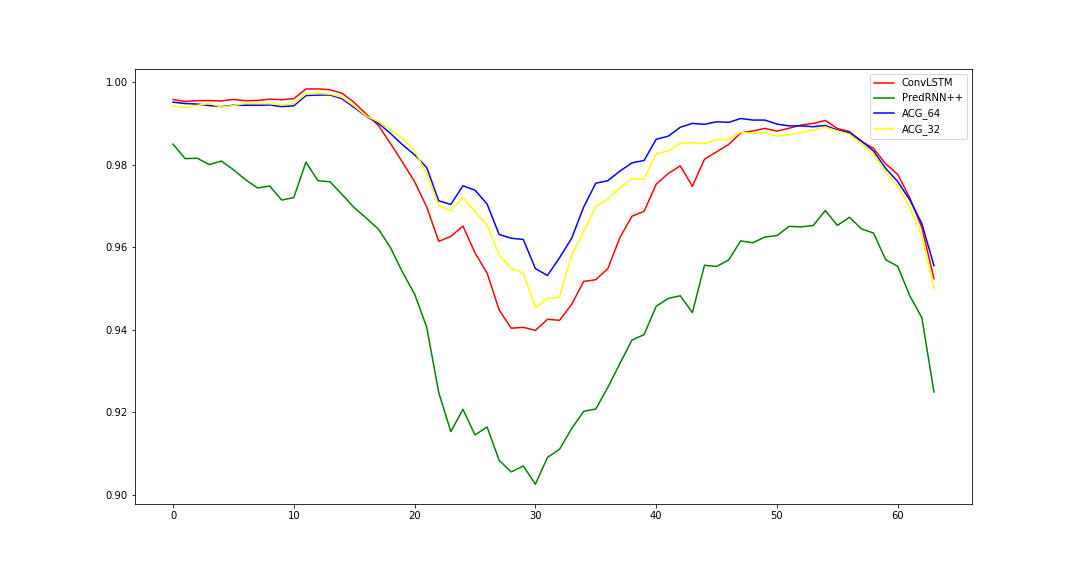
\includegraphics[width=.4\linewidth]{figures/chap4/recall_all_tests.png} \\
              \small Recall
          \end{tabular} 
          \begin{tabular}[b]{c}
              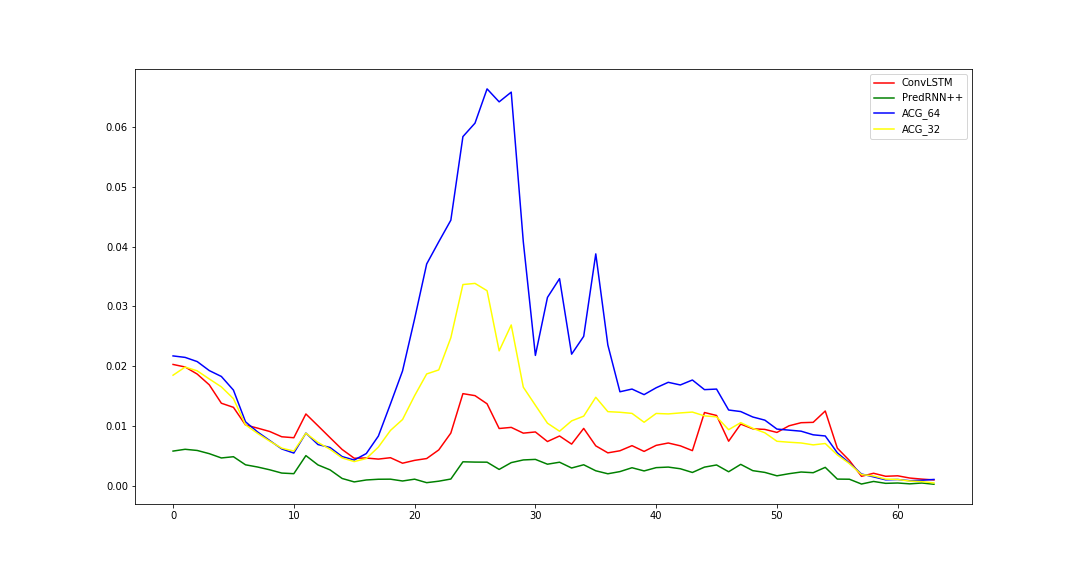
\includegraphics[width=.4\linewidth]{figures/chap4/fdr_all_tests.png} \\
              \small FDR
          \end{tabular}
    \end{center}
    \caption[]{Performance of all methods at all tests}
    \label{fig:chap4-performance-all-tests}
\end{figure}

Figure \ref{fig:chap4-performance-all-tests} indicates the performance of all methods in all metrics at all tests. The visualization shows that all methods yeild worse results in tests 25 to 35, which are from July to September. This time is in the wet season at Mekong Region %cite Water balance analysis for the Tonle Sap Lake–floodplain system
, where flooding and the associated water level increase in the Mekong River causes the Tonle Sap River to change flow direction and flow towards the northwest (upstream) into Tonle Sap Lake (see Figure ).

\begin{SCfigure}
    \caption[]{Monthly average water level of Tonle Sap Lake at Kampong Luong (continuous line – right vertical axis) and inundated area (circles – left vertical axis). The observed minimum and maximum monthly average water levels have been illustrated with dotted bars}
    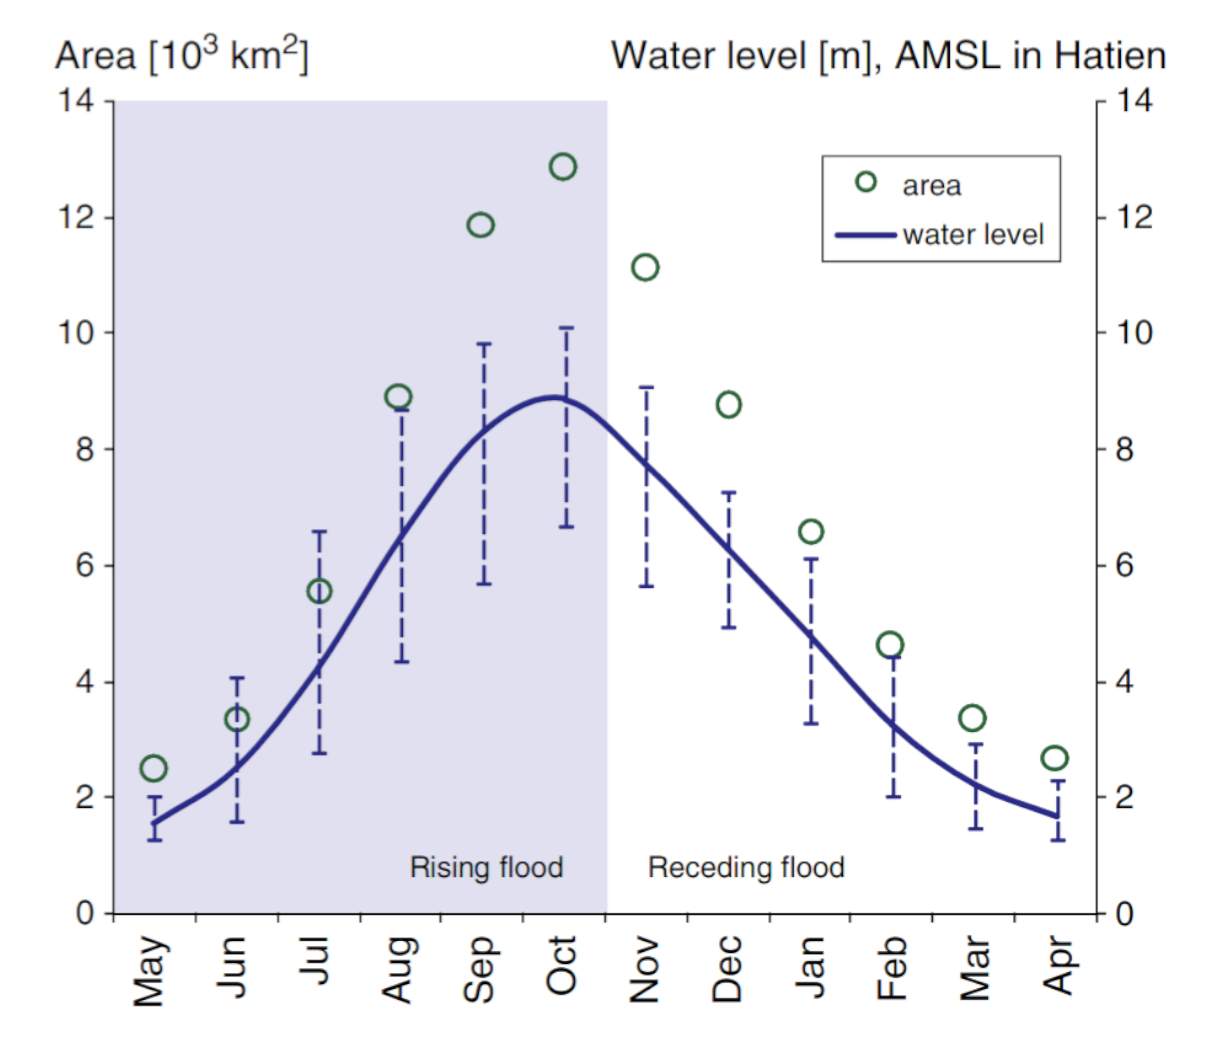
\includegraphics[width=.65\textwidth]{figures/chap4/tonlesap_avg_area_with_floodplain.png}
    \label{fig:chap4-tonlesap-avg-area}
\end{SCfigure}


\section{Conclusions}

